\documentclass{math}

\usepackage{graphicx}

\title{Introduction to Cryptography}
\author{Alvin Lin}
\date{January 2018 - May 2018}

\begin{document}

\maketitle

\section*{Block Ciphers}
A stream cipher algorithm defines how to encrypt or decrypt arbitrary length
messages. A block cipher can only encrypt or decrypt \( b \) bits, no more, no
less. Arbitrary length message are handled by a separate algorithm called a
block cipher mode of operation (ECB). A stream cipher's encryption and
decryption operations are the same. A block cipher's encryption and decryption
operations are different. To decrypt, the encryption operation must be run
backward. Thus, the encryption operation must be invertible. Additionally, block
ciphers are much more than just an encryption algorithm, they can be used:
\begin{itemize}
  \item to build different types of block-based encryption schemes
  \item to realize stream ciphers
  \item to construct hash functions
  \item to make message authentication codes
  \item to build key establishment protocols
  \item to make a pseudo-random number generator
\end{itemize}

\subsection*{Block Cipher Primitives}
Claude Shannon: there are two primitive operations with which strong encryption
algorithms can be built.
\begin{enumerate}
  \item \textbf{Confusion:} An encryption operation where the relationship
  between the key and ciphertext is obscured. Today, a common element for
  achieving confusion is substitution, which is found in both AES and DES.
  \item \textbf{Diffusion:} An encryption operation where the influence of one
  plaintext symbol is spread of over many ciphertext symbols with the goal of
  hiding statistical properties of the plaintext. A simple diffusion element is
  the bit permutation, which is frequently used within DES. This obscures the
  relationship between the ciphertext and the plaintext.
\end{enumerate}
Both operations by themselves cannot provide security. The idea is to
concatenate confusion and diffusion elements to build so called product ciphers.
Most of today's block ciphers are product ciphers as they consist of rounds
which are applied repeatedly to the data. This can reach excellent diffusion, as
changing one bit of the plaintext results on average in the change of half the
output bits.

\subsection*{Block Cipher Modes of Operation}
There are several ways of encrypting long plaintexts with a block cipher:
\begin{itemize}
  \item Electronic Code Book mode (ECB)
  \item Cipher Block Chaining mode (CBC)
  \item Output Feedback mode (OFB)
  \item Cipher Feedback mode (CFB)
  \item Counter mode (CTR)
  \item Galois Counter Mode (GCM)
\end{itemize}
These modes have the goal of providing authenticity and integrity in addition to
confidentiality. It ascertains that the message is coming from the original
sender and that it was not altered during transmission.

\subsubsection*{Electronic Code Book mode (ECB)}
This is the simplest of the encryption modes. Messages which exceed \textit{b}
bits are partitioned into \textit{b}-bit blocks, which are encrypted separately.
In case the plaintext message's length is not a multiple of \textit{b}, we add
padding to the end.
\begin{center}
  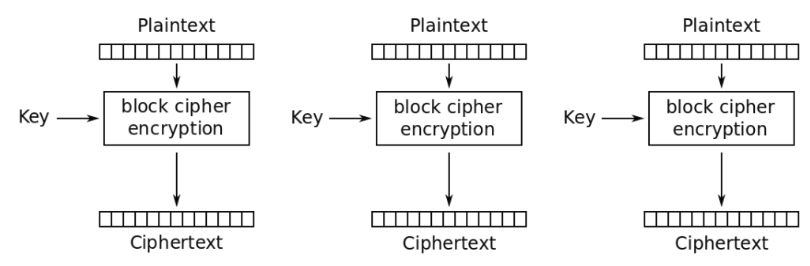
\includegraphics[width=12cm]{assets/ecb.png}
\end{center}
\textbf{Advantages:}
\begin{itemize}
  \item No block synchronization between the sender and receiver is required.
  \item Bit errors caused by noisy channels only affect the corresponding block
  but not succeeding blocks.
  \item Encryption can be parallelized, which is an advantage for high-speed
  implementations.
\end{itemize}
\textbf{Disadvantages:}
\begin{itemize}
  \item Encryption is highly deterministic.
  \item Identical plaintexts result in identical ciphertexts.
  \item An attacker recognizes if the same message has been sent twice.
  \item Plaintext blocks are encrypted independently of previous blocks.
  \item An attacker may reorder ciphertext blocks which result in valid
  plaintext.
  \item Statistical properties in the plaintext are preserved in the
  ciphertext.
\end{itemize}
Once a particular plaintext to ciphertext block mapping is known, a sequence of
ciphertext blocks can easily be manipulated.

\subsubsection*{Cipher Block Chaining mode (CBC)}
There are two main ideas behind this mode: the encryption of all blocks are
chained together, and the encryption is randomized by using an initialization
vector.
\begin{center}
  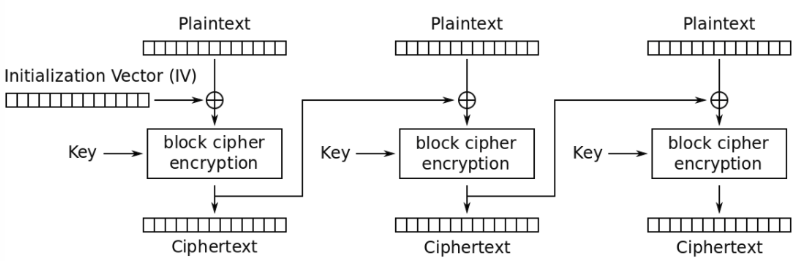
\includegraphics[width=12cm]{assets/cbc.png}
\end{center}
This mode also requires padding, but messages longer than \( 2^{\frac{n}{2}} \)
blocks (where \( n \) is the block size in bits) shouldn't be encrypted with
this mode, since it gives an attacker more information about the ciphertext.
Encryption cannot be parallelized, but decryption can be. The initialization
vector does not need to be secret, but it should be a randomized nonce.

\subsubsection*{Output Feedback mode (OFB)}
This mode builds a synchronous stream cipher from a block cipher, where the key
stream is generated in a blockwise fashion. The output of the cipher gives us
key stream bits with which we can encrypt plaintext bits using the XOR
operation. This mode also requires an initialization vector (which also should
be a randomized nonce).
\begin{center}
  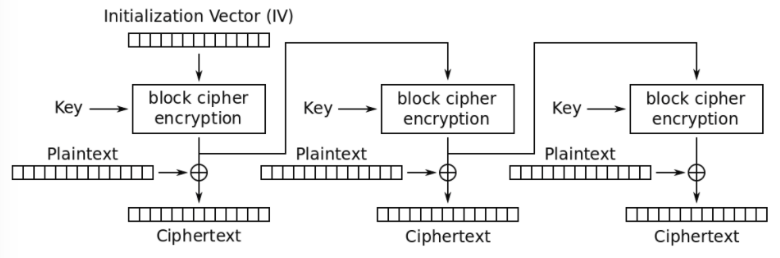
\includegraphics[width=12cm]{assets/ofb.png}
\end{center}

\subsubsection*{Cipher Feedback mode (CFB)}
This mode uses a block cipher as a building block for an synchronous stream
cipher. The key stream is generated in a blockwise fashion and is also a
function of the ciphertext. Since it also uses a randomized initialization
vector, the ciphertext is also nondeterministic. It can be used in situations
where short plaintext blocks are to be encrypted, but has no real advantage
over Output Feedback mode.
\begin{center}
  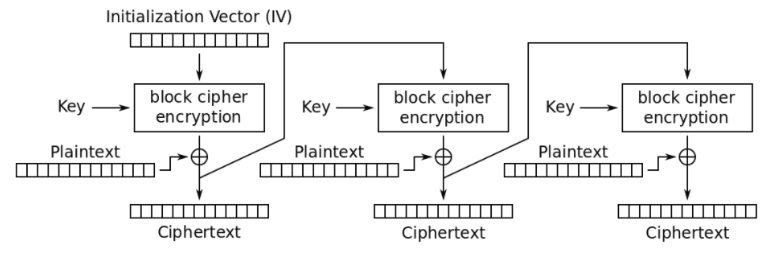
\includegraphics[width=12cm]{assets/cfb.png}
\end{center}

\subsubsection*{Counter mode (CTR)}
This mode turns a block cipher into a stream cipher where the keystream is
computed in a blockwise fashion (similar to OFB and CFB mode). The input to the
block cipher is a counter which assumes a different value every time the block
cipher computes a new key stream block. Unlike CFB, and OFB however, this is
highly parallelizable and does not require padding since the unneeded portion
of the last key block can be discarded (because it is a stream cipher).
\begin{center}
  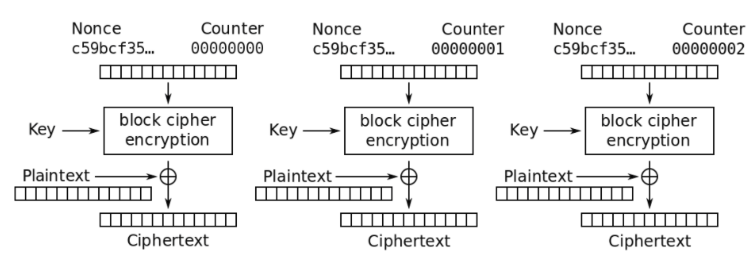
\includegraphics[width=12cm]{assets/ctr.png}
\end{center}

\subsection*{Feistel Cipher (Feistel network)}
Horst Feistel proposed the use of a cipher that alternates substitutions and
permutations. This is a practical application of a proposal by Claude Shannon to
develop a product cipher. A large set of block ciphers use the scheme (it is a
design model from which many different block ciphers are derived), including the
Data Encryption Standard (DES). DES is just one example of a Feistel Cipher.

\subsection*{Data Encryption Standard (DES)}
\begin{itemize}
  \item Data Encryption Standard (DES) encrypts blocks of size 64 bit.
  \item Developed by IBM based on the cipher Lucifer under the influence of the
  National Security Agency (NSA).
  \item Standardized in 1977 by the National Bureau of Standards (NBS), now
  called the National Institute of Standards and Technology (NIST).
  \item Most popular block cipher for most of the last 30 years.
  \item By far the best studied symmetric algorithm.
  \item Nowadays considered insecure due to the small key length of 56 bits.
  \item Replaced by the Advanced Encryption Standard (AES) in 2000.
\end{itemize}
By encrypting with DES three times in a row, triple DES (3DES) was created,
against which no practical attack is currently known. 3DES is still widely in
use today.

\subsubsection*{DES Algorithm Internals}
The DES algorithm is a symmetric cipher that encrypts 64-bit blocks using a
56-bit key. It performs 16 rounds of operations on the plaintext, performing
the following sequence of operations 16 times:
\begin{enumerate}
  \item \textbf{Expansion function \( E \):} increases diffusion by taking the
  32 input bits and duplicating some to fit them into a 48 bit block.
  \item \textbf{XOR with round key:} the 48-bit block is XOR'ed with a 48-bit
  round subkey. A different subkey derived from the main key is used in each
  round.
  \item \textbf{Substitution using S-boxes:} the 48-bit block is split into 8
  chunks that are 6 bits long and a predetermined \( 4\times16 \) substitution
  box is used to translate the 6-bit input into a 4-bit output. The first and
  last bit determine the row of the substitution box to use while the middle
  four bits determine the column of the substitution box to use. This is the
  S-box used in round one of the DES algorithm:
  \begin{center}
    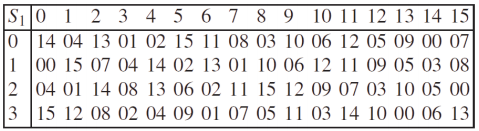
\includegraphics[width=8cm]{assets/sbox.png}
  \end{center}
  The bit sequence 100101 would be substituted with the entry in row 11 (4 in
  decimal) and column 0010 (3 in decimal). Using the S-box above, this would be
  the value 08 (1000 in binary). The S-boxes are crucial for DES security since
  they introduce a non-linear element, making this algorithm resistant to
  differential analysis.
  \item \textbf{Permutation:} a bitwise permutation is performed to introduce
  diffusion. The sum of all these operations ensures that after round 5, every
  bit of output is a function of each key bit and each plaintext bit.
\end{enumerate}
\begin{center}
  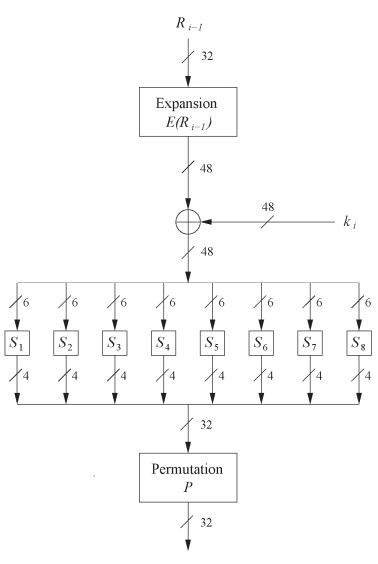
\includegraphics[width=8cm]{assets/des_round.png}
\end{center}
Because DES is a Feistel Cipher, only the key schedule needs to be modified for
decryption. The round subkeys need to be generated in reverse order, and after
that the encryption algorithm can be applied using the keys in reverse to
decrypt the data.

\subsubsection*{Analytical Attacks}
DES is quite robust against known analytical attacks such as linear and
differential analysis. In practice, it is very difficult to break the cipher
with linear or analytical cryptanalysis.

\subsubsection*{Exhaustive Key Search}
A simple exhaustive search for a DES key pair knowing one plaintext-ciphertext
pair is relatively easy given today's computer technology since DES has a key
space of size \( 2^{56} \). However, for most other block ciphers, a key search
is somewhat more complicated. A brute-force attack can produce false positive
results, where a key is found that is not the one used for the encryption. The
likelihood of this is related to the relative size of the key space and the
plaintext space. \par
Assume a cipher with a block width of 64 bits and a key size of 80 bits is used
to encrypt a plaintext. If we encrypt once under all possible \( 2^{80} \) keys,
we obtain \( 2^{80} \) possible ciphertexts. However, there exist only
\( 2^{64} \) different ones. If we run through all keys for a given
plaintext-ciphertext pairs, we find on average \( \frac{2^{80}}{2^{64}} =
2^{16} \) keys that perform the mapping \( e_k(x) = y \). Given a block cipher
with a key length of \( k \) bits and a block size of \( n \) bits, as well as
\( t \) plaintext-ciphertext pairs, the expected number of false keys which
encrypts all plaintexts to the corresponding ciphertexts is \( 2^{k-tn} \).

\subsection*{Advanced Encryption Standard (AES)}
\begin{itemize}
  \item AES is the most widely used symmetric cipher today
  \item The algorithm for AES was chosen by the US National Institute of
  Standards and Technology (NIST) in a multi-year selection process, requiring
  all AES candidate submissions to be block ciphers with 128-bit block sizes
  supporting 128-bit, 192-bit, and 256-bit keys.
  \item 5 finalists were announced in August 1999:
  \begin{itemize}
    \item \textit{Mars} - IBM Corporation
    \item \textit{RC6} - RSA Laboratories
    \item \textit{Rijndael} - J. Daemen and V. Rijmen
    \item \textit{Serpent} - Eli Biham et al.
    \item \textit{Twofish} - B. Schneier et al.
  \end{itemize}
  \textit{Rijndael} was chosen as the new AES in October 2000 and formally
  approved as a US federal standard in November 2001.
  \item Like DES, AES operates by applying rounds of operations to the
  plaintext. The number of rounds performed depends on the key length.
  \begin{center}
    \begin{tabular}{|c|c|}
      \hline
      Key length (bits) & Number of rounds \\ \hline
      128 & 10 \\ \hline
      192 & 12 \\ \hline
      256 & 14 \\ \hline
    \end{tabular}
  \end{center}
\end{itemize}

\subsubsection*{AES Algorithm Internals}
The AES algorithm is a byte-oriented cipher, so the 128-bit cipher text is
arranged into a \( 4\times4 \) matrix of bytes. Each round consists of layers,
which perform the following operations on the matrix:
\begin{enumerate}
  \item \textbf{Byte Substitution Layer:} 16 identical S-boxes are used to map
  each byte in the matrix to some new value. These S-boxes are the only
  nonlinear elements of AES and are bijective, so they can be uniquely reversed.
  \item \textbf{Diffusion Layer:} the input state bits are passed through two
  sub-layers:
  \begin{itemize}
    \item \textbf{ShiftRows Sublayer:} a bytewise permutation is performed,
    which left shifts the first row of the matrix once, left shifts the second
    row twice, and left shifts the third row three times.
    \item \textbf{MixColumn Sublayer:} each 4-byte column of the matrix is
    multiplied by some fixed \( 4\times4 \) matrix to mix each column of the
    state matrix.
  \end{itemize}
  This layer provides diffusion over all the input state bits.
  \item \textbf{Key Addition Layer:} the 16-byte state matrix is XOR'ed with a
  16-byte subkey generated in the key schedule, derived from the original
  input key.
\end{enumerate}
This process is reversed for decryption. Since AES is not based on a Feistel
network, all the layers must be reversed for decryption. Generally, this means
that all the subkeys must be conputed before the decryption of the first block
can begin.

\subsubsection*{Implementation in Software}
NIST also required that AES had the possibility of an efficient software
implementation. A straightforward implementation is well suited for 8-bit
processors, but inefficient on 32-bit and 64-bit processors. A more
sophisticated approach would be to merge all the layer functions except the
key addition into a table lookup, allowing a round to be computed using 16 table
lookups.

\subsubsection*{Security}
Due to the key length, a brute force attack is infeasible. There exist no known
analytical attacks, but several side-channel attacks have been published. These
attacks target implementations of the algorithm however, rather than weaknesses
in the underlying algorithm.

\begin{center}
  You can find all my notes at \url{http://omgimanerd.tech/notes}. If you have
  any questions, comments, or concerns, please contact me at
  alvin@omgimanerd.tech
\end{center}

\end{document}
